\documentclass[10pt, twoside]{extarticle}

% TeX gyre pagella fonts
\usepackage{mathptmx}
\usepackage{enumitem}
\usepackage{tikz}
\usepackage{marvosym} % \Email
\usepackage[affil-it]{authblk}
\usetikzlibrary{trees}
\usepackage{microtype}
\usepackage{minted}
\usepackage{lipsum}
\usepackage{csquotes}
\usepackage{xcolor}
\usepackage{movie15}
\usepackage[document]{ragged2e}

\usepackage[paper=a4paper,margin=1.45in]{geometry}
\usepackage[colorlinks=true]{hyperref}

\def\changemargin#1#2{\list{}{\rightmargin#2\leftmargin#1}\item[]}
\let\endchangemargin=\endlist 
\hypersetup{
  citecolor=black,
  linkcolor=blue,
  urlcolor=blue
}
\begin{document}
% \thispagestyle{plain}
\begin{center}
    \vspace*{20mm} 
    \Huge
    Toward a User Friendly JuliaImages
        
    \vspace{0.4cm}
    \large
    Google Summer of Code 2021 Proposal
        
    \vspace{1.0cm}
    \textbf{Ashwani Rathee}
    
    \vspace{0.2cm}
    \href{ashwani.198023@gmail.com}{ab669522@gmail.com}
    
    \vspace{1.0cm}
    April 2021
       
    \vspace{0.9cm}
    \textbf{Abstract}

    \vspace{0.2cm}
    \begin{changemargin}{1.5cm}{1.5cm} 
    \large
    \begin{flushleft}
     JuliaImages is a state of the art image processing
ecosystem available to the community. Being written purely in
Julia and having a huge number of algorithms - this ecosystem provides both almost-complete and easy interface environment for users.  Being said that,
there is lack of organized setup for worked out demonstrations. There are several mini examples scattered around in
the documentation of various packages in JuliaImages. This project
aims to solve this very issue by organising the examples, reworking
the current examples and adding a good number of new examples.
    \end{flushleft}   
    \end{changemargin}
\end{center}

% This project aims to improve the visibility of the various image processing packages provided by JuliaImages and move toward a more beginner friendly JuliaImages with increased Visualization and Interactivity tools.Main contributions consist of making demos for various Image processing functionalities available and improving on ImageDraw.jl and ImageView.jl.
\Huge
\textsf{1.  Description of the Project}\\

\vspace{0.5cm}
\large
Image Processing is an important part of science. Image processing plays a very important role in science from helping Hubble telescope to explore the wide universe, to helping researchers segment HeLa cells. JuliaImages is one of the most feature rich and optimized ecosystems for solving image processing problems. Performance has always been a top priority for this ecosystem. It is highly optimized towards memory and speeds given the clean architecture and efficient code design. But still, there is not yet a well organized set of demonstrations to allow new and experienced users to explore capabilities of JuliaImages similarly with well-written clear and concise demonstrations. Here I propose ideas on how the 
growth of this ecosystem can be further fueled by this project which focuses on the addition of new fully-worked out examples, reworking old examples and organising them under \textbf{Demonstrations}.



\newpage
\newgeometry{margin=1.3in}
\Large
{}{1.1 Project : Improved Demonstrations Section}

\vspace{0.5cm}
\large
JuliaImages ecosystem hosts numerous packages that provide equivalently\\ complete set of highly performant algorithmic features as provided by scikit-image, opencv, and MatLab image processing frameworks.  \\

Images.jl is an umbrella package that exports a set of packages that are useful for common image processing tasks.One particular line that caught me attention :
\begin{displayquote}
"Elements of this package descend from "image.jl" that once lived in Julia's extras/ directory. That file had several authors, of which the primary were Jeff Bezanson, Stefan Kroboth, Tim Holy, Mike Nolta, and Stefan Karpinski."

\end{displayquote}

From image.jl to the widespread JuliaImages,that's a impressive story of persistence I think . I would like to be part of it in some way.

\vspace{0.5cm}
\Large
\underline{Overview of the project}

\vspace{0.3cm}
\large
The main motivation for this project is that lack of examples create a gap between the user of JuliaImages and the plethora of capabilities provided by JuliaImages. Even though the doc string of the algorithms provided by the developers are well written in most cases, but still docstring cannot replace the online demonstrations for easy and quick usage examples.

\vspace{0.5cm}
\Large
\underline{Current Status}

\vspace{0.3cm}
\large
Demonstrations section made with Democards.jl currently holds 12 examples and several others scattered in particular package documentations.

In Demonstrations :
\begin{itemize}[noitemsep,topsep=0.2cm]
    \item 4 related to general handling of image data
    \item 4 related to spatial transformations
    \item 3 related to contours
    \item 1 related to quality indexes
\end{itemize}
7 tutorials are currently present in ImageFeatures.jl docmentation.2  demonstrations are present in ImageFiltering.jl documentation. Demonstrations of algorithms are present in ImageSegmentation.jl all cluttered in one page.
% \large
% Packages can be divided into 3 types of packages as shown below:\\
% 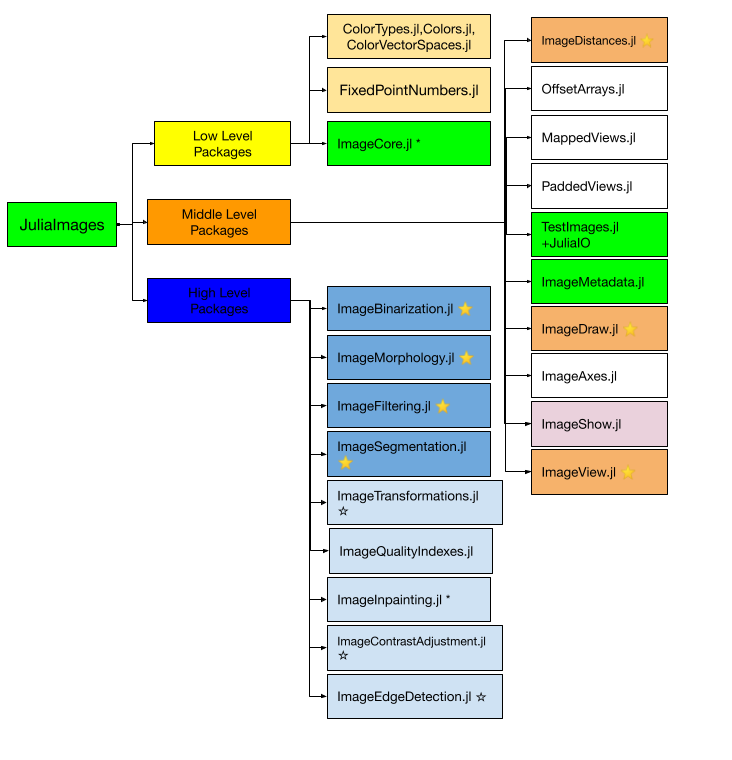
\includegraphics[scale=0.6]{assets/Pathi.png}
% Currently, Packages under JuliaImages can be roughly categorised into 3 types :
% \begin{itemize}[noitemsep,topsep=0pt]
%     \item High level packages
%     \item Middle level packages
%     \item Low level packages
% \end{itemize}

% 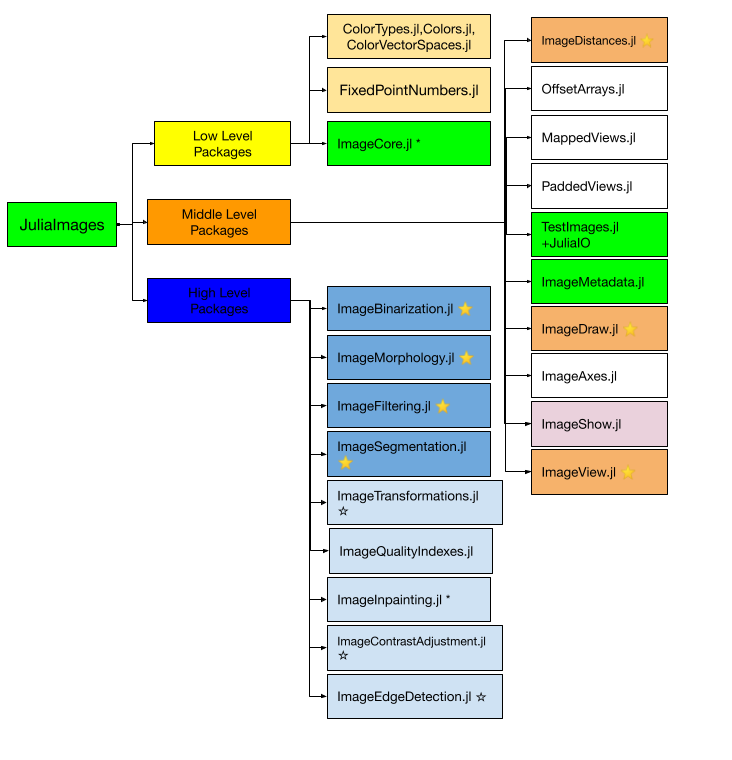
\includegraphics[scale=0.4]{assets/Pathi.png}

\vspace{0.5cm}
\Large
\underline{Project Details}

\vspace{0.5cm}
\large
Project is divided in 4 sections:
\begin{itemize}[noitemsep,topsep=0.2cm]
    \item Section 1: Demonstrations on Image Binarization and Morphology
    \item Section 2: Demonstrations on Image Features
    \item Section 3: Demonstrations on Image Segmentation
    \item Section 4: Demonstrations on Image Quality Indexes and Contrast Adjustment
\end{itemize}
According to the current project plan, most of the work for first 2 sections should be completed before the first evaluation and similarly section 3 and section 4 work would be done in week 6-10. Since the work done in any open source community is asynchronous,so some demonstrations/ideas might take longer to get merged/added depending on the reviews,feedback and updating the PRs with according to the feedback.\\
With this current project plan,12-14 demonstrations will be added covering most of capabilities in ImageBinarization.jl, ImageMorphology.jl, ImageSegmentation.jl, ImageQualityIndexes.jl and ImageFeatures.jl packages. 

% \vspace{0.3cm}
% Providing the users with example.jl and pluto/jupyter notebook in .jl/.ipynb format for download directly on JuliaImages website  or providing them the tutorials in github repositories.

Project will be discussed in more details with my mentor in community bonding period.

\vspace{0.3cm}
\textbf{Note: }There are several projects in JuliaImages like ImageTransformations.jl, ImageFiltering.jl and from people in Julia's image processing like ImageProjectiveGeometry.jl, Augmentor.jl  that haven't been touched in this project, so those might be potential demonstrations ideas for the community bonding period and of course in post GSOC period. There are several low level packages and utilities package like ImageDraw.jl,ImageView.jl, TiledIteration.jl that haven't been covered in this project plan due to time constraints and delivering limited quantity-high quality work.
% \vspace{0.5cm}
% High Level Packages in JuliaImages includes:
% \begin{itemize}[noitemsep,topsep=0]
%     \item ImageBinarization.jl provides various image binarization algorithms.
%     \item ImageContrastAdjustment.jl supports image contrast enhancement and manipulation.
%     \item ImageMorphology.jl provides several morphological operations for image processing.
%     \item ImageFiltering.jl supports basic filtering operations.
%     \item ImageFeatures.jl is a package for identifying and characterizing "keypoints" (salient features) in images.
%     \item ImageQualityIndexes.jl provides several image quality assessment indexes, e.g., PSNR and SSIM.
%     \item ImageTransformations.jl provides functions related to geometric transformations.
%     \item ImageSegmentation.jl provides several image segmentation algorithms.
%     \item ImageInpainting.jl provides image inpainting algorithms in Julia
% \end{itemize}

% \vspace{0.5cm}
% \Large
% \underline{Images.jl}

% \vspace{0.5cm}
% \large

% Images.jl is an "umbrella package" that exports a set of packages that are useful for common image processing tasks. \\
% The author has good storytelling to emphasize the importance of this package.
% One particular line that shows how it has grown over years:\\

% \\
% Images.jl quite literally has a ton of functions since it exports almost all functions in JuliaImages all at once.

% According to the project plan, It al implement 12 - 14 demos(depends on if we wish to combine multiple operations in a single demo, and how compact we want the demos and functions in them to be). I'll go into detail about which part deserves space on the demos section of JuliaImages with help of DemoCards.jl.I will go into the discussion for each package provided and where it fits in demos.
% \subsection{Review with analysis for demos}
% \newpage

\vspace{0.5cm}
\Large
\textbf{\textsc{1.1 Section 1: Demonstrations on Image Binarization and Morphology}}


\vspace{0.5cm}
\Large
\textsf{ImageBinarization.jl + HistogramThresholding.jl}\\

\vspace{0.5cm}
\large
These packages mainly provide algorithms to convert grayscale images into black\\ or white(binary image). Image binarization is one of the most important steps in \\pre-processing of images to save all or maximum sub-components such as objects, text, background, and image.\\
Histogram Thresholding also provides similar functionalities and a little more in terms of abilities to get more than black or white. Long demonstration will come from this section.
\\
There are currently 12 algorithms available to perform image binarization/thresholding:
\begin{itemize}[noitemsep,topsep=0pt]
    \item Some Algorithms perform better for text data i.e. Niblack and Sauvola
    \item Some Algorithms perform better for distinct contrast between foreground and background i.e. Adaptive Threshold
\end{itemize}

Points to be covered:
\begin{itemize}[noitemsep,topsep=0pt]
    \item  What if I don't know which one is best algorithm for my specific use case?How to check that fast?
    \begin{displayquote}
    \begin{minted}{julia}
    function binarize_methods()
    . 
    .
    end
    \end{minted}
    By using this function, which applies all the methods to test image and shows all of them in one place with MosaicViews.jl
    \end{displayquote}
    \item Cases for 2-D and 3-D images
    \begin{displayquote}
    For the 3-D case, we can use ImageView.jl to show the effect in the 3-D image to the viewer.
    \end{displayquote}
    \item Cases for textual and high contrast images need to be taken,\\to show Niblack and Sauvola use cases.
    \item For simpler methods, we can use simple linear gradients to effectively show what those methods do \\
     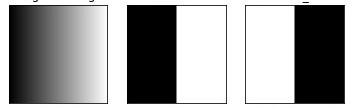
\includegraphics[]{assets/1.png}
    \begin{displayquote}
   
    \end{displayquote}
\end{itemize}


\vspace{0.5cm}
\Large
\textsf{ImageMorphology.jl}

\vspace{0.5cm}
\large
ImageMorphology.jl exports JuliaImages's collection of non-linear operations related to the shape or morphology of features in an image.

\begin{enumerate}
  \item  Basic methods : Erosion, Dilation, Closing, Tophat, Bothat, Morphological Gradient, Morphological Laplace 
  \item  Other methods : convexhull, imfill(for small holes filling), clearborder(to clear image's border), thinning algorithm.
\end{enumerate}
 2 Long demonstrations: One of basic methods, and other to show usage of convex hull, image hole fill, clear border, thinning.
 \begin{enumerate}
     \item Long Example : Implementation of the basic algorithms and then comparing the results with the other results and discussion on how the threshold of Gray affect the performance.
     \begin{minted}{julia}
     img_erosion = erode(Gray.(img) .< 0.7)
     \end{minted}
     \begin{displayquote}
        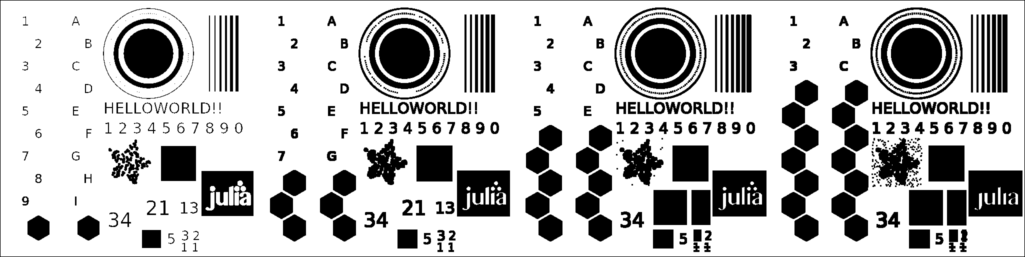
\includegraphics[width=10cm,scale=0.5]{assets/morphology.png}
     \end{displayquote}
     \item Long Example with usage of convexhull, image fill, thinning, clear border and usage of polygon filling algorithm after convex hull points extraction
     \begin{displayquote}
        Input image would be the image of a coin with unclear border, noisy with Noise.jl
     \end{displayquote}
    \item Emphasis on input methods and conversion, since some of the above methods only take boolean images.
    \item Emphasis on creation of boolean image from RGB and GRAY image using thresholding and visualizing them properly afterward
 \end{enumerate}

To effectively show the capabilities of the Image Binarization and Morphology with Democards for 3d Image, Democards.jl should be able to effectively show 3d image which is not the case yet. So in the community period,this problem also needs to be resolved.

\vspace{0.5cm}
\Large
\textbf{\textsc{1.2 Section 2: Demonstrations on Image Features}}

\vspace{0.5cm}
\Large
\textsf{ImageFeatures.jl}

\vspace{0.5cm}
\large
This package is used to identify and characterize key points in images.\\
The collection of key points can be matched between two images as shown in the tutorials.\\

There are 7 tutorials currently available in ImageFeatures.jl that need to be transferred to the demonstrations section and they need some bug fixing. GLCM and Local Binary Pattern tutorials need to be reworked/created. 

\vspace{0.5cm}
Points to be covered :
\begin{enumerate}
    \item  BRIEF, ORB, FRISK, Object detection using HOG, FREAK, Local Occurrence Matrix, Local Binary Patterns need to be transferred to Demonstrations section and reworking them to be more concise.
    \item BRIEF examples need to be updated with test images other than Lena. ORB, FRISK, BRISK has issues with output calculation due to RotMatrix since Rotations.jl isn't imported.
    \item Show the differences in performances of these algorithms for a image and compare results.
    \item Show how these algorithms approach a problem like FREAK,BRISK has defined sampling pattern.In BRISK,pixels are sampled over concentric rings and FREAK approaches it differently.
    \begin{displayquote}
        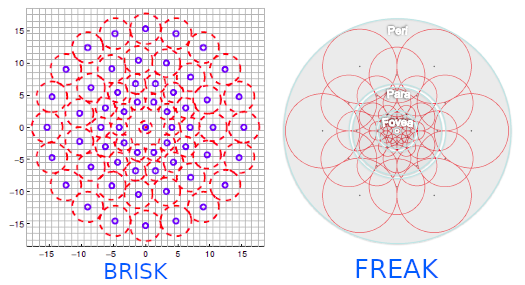
\includegraphics[width=10cm,scale=0.5]{assets/image (1).png}
     \end{displayquote}
    \item Demonstration on GLCM Texture Analysis :
    \begin{itemize}
        \item How to create a GLCM matrix and how matrix is related to image
        \item Using distance, angles for directional analysis in GLCM
        \item Deriving properties like correlation, variance, mean etc
        \item Use of symmetric version of GLCM
    \end{itemize}
    
    \item Long Demonstration on usage of local binary patterns 
    \begin{displayquote}
    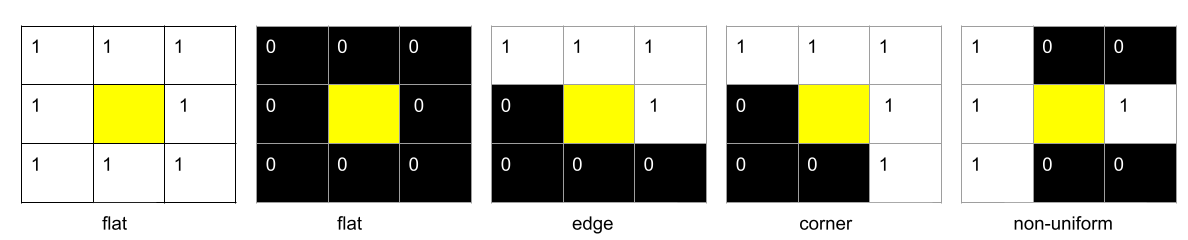
\includegraphics[width=10cm,scale=0.5]{assets/Untitled drawing (1).png}
    
       Use rotated images of faces, other objects at different orientations and then compare them and check if they are similar with Image differences methods
    \end{displayquote}
    \begin{itemize}
        \item Show how the LBP are calculated, computation of histogram from frequency of cells
        \item Show how LBP can be used in texture and pattern recognition
    \end{itemize}
\end{enumerate}

% \newpage
\vspace{0.5cm}
\Large
\textbf{\textsc{1.3 Section 3: Demonstrations on Image Segmentation}}

\vspace{0.5cm}
\Large
\textsf{ImageSegmentation.jl}

% https://scikit-image.org/docs/dev/user_guide/tutorial_segmentation.html
% https://juliaimages.org/stable/pkgs/segmentation/
\vspace{0.5cm}
\large
This package provides the algorithms related to segmentation of images. Although documented quite extensively in the documentation, it needs to be broken into short demo pieces that are quick,concise to use for a new user.\\
Most of the demos can be considered under the reworking section since they are pretty well documented but needs to be broken down into pieces.\\
Since this part needs a lot of repetitive work, there is need to discuss on where the emphasis should on certain part of the algorithms.\\ 
For example : In watershed segmentation, the distance to the background is calculated which should be emphasised on.\\

Points to be covered :
\begin{itemize}[no 5titemsep,topsep=0]
    \item Watershed Segmentation Algorithm
    \begin{itemize}
        \item Focus on showing distance transform,labelcomponents,labelsmap and showing segmentation accuracy with various degree grayscale images
    \end{itemize}
    \item Seeded + Unseeded Region Growing Algorithm
    \begin{itemize}
        \item Emphasis on suitable selection of seed points, minimum area threshold, similarity threshold value is important
    \end{itemize}
    \item Felzenswalb's Region Merging Algorithm
        
    \item Mean Shift Segmentation Algorithm
    \begin{itemize}
        \item Emphasis on how meanshift doesn't scale well with size of image and why we use iters,eps keywords,how kernel size i.e. spatial radius,range radius affects resolution of mode detection
    \end{itemize}
    \item Fast Scanning Segmentation Algorithm
    \begin{itemize}
        \item Emphasis on how fast it can be and how choice of threshold affects results
    \end{itemize}
    \item Fuzzy C-means,K-means Algorithm
    \item Creating Region Adjacency Graphs
    \item Creation of Region Trees and Region Splitting using RegionTrees
\end{itemize}

\vspace{0.3cm}
Also, Comparison demonstration/tutorial of these segmentation and superpixel algorithms would also improve the user's understanding on how and where a particular algorithm would be most efficient.

% \newpage
\vspace{0.5cm}
\Large
\textbf{\textsc{1.4 Section 4: Demonstrations on Quality Indexes and\\ Contrast Adjustment}}

\vspace{0.5cm}
\Large
\textsf{ImageContrastAdjustment.jl}

\vspace{0.5cm}
\large
This package provides algorithms for contrast adjustments.
Most of its \\ exported functions use cases are shown in histogram equalization example and \\histogram matching example.\\

A good idea would be to rework both the histogram matching demo and histogram \\equalization demo to more accurately show
\\
Points to be covered:

\begin{itemize}
    \item Use a different test image than moon surface, probably  mountain stream png or lakecolor tiff, as they will be more clearly able to show how gamma correction among others can be used for
    images clicked in poor lighting conditions.
    
    \item Also,it would be a good idea to take a matrix and show the effect of all the algorithms in one place.
    \begin{displayquote}
       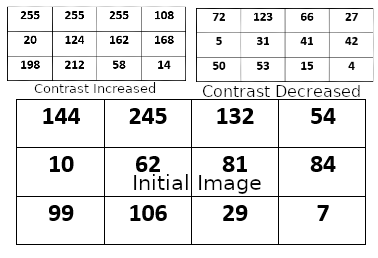
\includegraphics[scale=0.5]{assets/contrast.png}
    \end{displayquote}
    \item Also, examples need to be reworked to show the histogram calculated through buildhistogram functionality
\end{itemize} 

% \href{http://learningjulia.com/2017/03/09/imfilter-and-arrays.html}{Imfilter Example}\\
% \href{http://learningjulia.com/2017/02/24/blurring-and-manipulation.html}{Blurring and ImageManipulation}

% Demonstration of filtering kernels needs to be discussed
% #TODO



\vspace{0.5cm}
\Large
\textsf{ImageQualityIndexes.jl}

\vspace{0.5cm}
\large
ImageQualityIndexes provides the basic image quality assessment methods.
There are currently 3 methods that return ratios:
\begin{itemize}
    \item Peak signal-to-noise ratio
    \item Structural similarity
    \item Multi-scale SSIM
    \item Colorfulness
\end{itemize}
Even though SSIM has a good demonstration already available on the website, we should make a QualityIndexes Complete example for a movie-like array of Images using ImageView.jl as shown in its documentation for human brain MRI.
Points to be covered:
\begin{itemize}
    \item All 4 Quality Indexes to be calculated for two movies(arrays of images) run side by side like shown below:
    \begin{displayquote}
       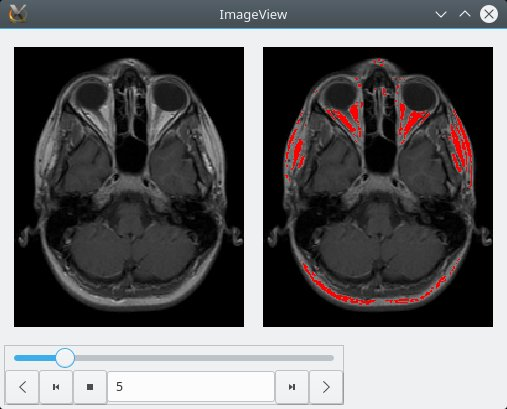
\includegraphics[scale=0.8]{assets/coupled.jpg}
    \end{displayquote}
\end{itemize}

\vspace{0.5cm}
\Large
\underline{ImageFiltering.jl}

\vspace{0.5cm}
\large
ImageFiltering.jl implements blurring, sharpening, gradient computation, and other linear filtering operations, as well as nonlinear filters like min/max.
ImageFiltering.jl provides 2 demos:
\begin{enumerate}
    \item Custom median filters (shows use of median filter with mapwindow)
    \item Max min filters(show use of min,max filter)
\end{enumerate}

These tutorials need to be moved to demonstrations section.
% \vspace{0.5cm}
% \Large
% \underline{ImageDistances.jl}

% % https://scikit-image.org/docs/dev/auto_examples/segmentation/plot_metrics.html#sphx-glr-auto-examples-segmentation-plot-metrics-py
% \vspace{0.5cm}
% \large
% Well I don't know it's use so it's quite a big fuckup here
% This 
% - https://scikit-image.org/docs/dev/auto_examples/segmentation/plot_metrics.html#sphx-glr-auto-examples-segmentation-plot-metrics-py
% -https://scikit-image.org/docs/dev/auto_examples/segmentation/plot_hausdorff_distance.html#sphx-glr-auto-examples-segmentation-plot-hausdorff-distance-py
% - https://scikit-image.org/docs/dev/auto_examples/transform/plot_ssim.html#sphx-glr-auto-examples-transform-plot-ssim-py
% -https://scikit-image.org/docs/dev/auto_examples/filters/plot_j_invariant_tutorial.html#sphx-glr-auto-examples-filters-plot-j-invariant-tutorial-py
% https://scikit-image.org/docs/dev/auto_examples/filters/plot_cycle_spinning.html#sphx-glr-auto-examples-filters-plot-cycle-spinning-py
% https://scikit-image.org/docs/dev/auto_examples/filters/plot_nonlocal_means.html#sphx-glr-auto-examples-filters-plot-nonlocal-means-py
% https://scikit-image.org/docs/dev/auto_examples/filters/plot_denoise_wavelet.html#sphx-glr-auto-examples-filters-plot-denoise-wavelet-py

% Euclidean,Sqlidean,CityBlock,TotalVariation,Minkowski,Hamming,SumAbsoluteDifference,SumSquaredDifference,MeanAbsoluteError,MeanSquaredError,RootMeanSquaredError,NCC,Hausdorff and Modified Hausdorff julia


% \vspace{0.5cm}
% \Large
% \underline{ImageTransformations.jl}

% \vspace{0.5cm}
% \large
% Exports     restrict,
%     imresize,
%     center,
%     warp,
%     WarpedView,
%     warpedview,
%     InvWarpedView,
%     invwarpedview,
%     imrotate

% - Translation  
% - Rotation
% - Affine Transformation
% - Perspective Transformation

% One example from this section https://scikit-image.org/docs/dev/user_guide/geometrical_transform.html
% https://scikit-image.org/docs/stable/auto_examples/transform/plot_geometric.html
% -can be used with imagefeatures.jl
% https://juliaimages.org/stable/pkgs/segmentation/
% https://juliaimages.org/v0.20/imagesegmentation/
% \href{https://juliaimages.org/stable/pkgs/segmentation/}{Link}. 
% \vspace{0.5cm}
% \Large
% \underline{ImageInpainting.jl}

% \vspace{0.5cm}
% \large
% This project is still under WIP, but it has Criminisi which is interesting, might be a good to increase its visibility
% Inpainting is a conservation process where damaged, deteriorating, or missing parts of an artwork are filled in to present a complete image.
% Currently, this package only provides Criminisi Examplar-based Algorithm.

% Since, Image InPainting and Image Restoration are similar fields with interests in restoring damaged/incomplete images for which JuliaImages doesn't have much functionality yet.

% Small Demo: It would be a good idea to make a small demo on this topic of course after combining it with other algorithms, we can use noisy images with small and major holes and distortions. This will help in further work in Image restoration algorithms.




% \vspace{0.5cm}
% \Large
% \underline{ImageTracking.jl}

% \vspace{0.5cm}
% \large
% ImageTracking.jl provides algorithms for object tracking,currently provided optical flow estimation with following algorithm: 
% \begin{enumerate}
%     \item Lucas-Kanade Algorithm(for sparse optical flow)
%     \item Farneback Algorithm(for dense optical flow)
% \end{enumerate}

% This project adds novel functionality but isn't mentioned in Julia images website and it has  
% Long demonstration can come from here:

% \begin{enumerate}
%     \item Demonstration of image registration using optical flow which shows how
% image registration uses optical flow and how image tracking in multiple happens?
% \end{enumerate}

% 	# main functions
%     optical_flow,
%     optical_flow!,

% 	# other functions
% 	haar_coordinates,
% 	haar_features,

% 	# other functions
% 	ColorBased,
% 	EndpointError,
% 	AngularError,
% 	polynomial_expansion,
% 	RasterConvention,
% 	CartesianConvention,
% 	visualize_flow,
% 	read_flow_file,
% 	evaluate_flow_error,
% 	calculate_statistics,

% 	# optical flow algorithms
% 	LucasKanade,
% 	Farneback,

%     # types that select implementation
%     ConvolutionImplementation,
%     MatrixImplementation
    
    % tracks and deserves a demo
% \vspace{0.5cm}
% \Large
% \underline{ImageEdgeDetection.jl}

% \vspace{0.5cm}
% \large
% This new package need to presented with demos in the main demo
% - Progress has already been made with Canny Edge Filter Demo written by me and reworked by Johnny Chen to fit specific needs
% - Although Now I feel that the usage of imgradients() and thinning algorithms can be shown in more details so, yeah I believe that the current demo can be improved to fit the needs for other as canny had different requirement than this

% -deprecating old canny
% -issues with hough transform
% - NEEDS REWORK WITH discussion of imgradients and thinning algorithms
% \section{Next Section}
% \subsection{ImageDraw.jl}

% ImageDraw supports basic drawing on Images. You can draw points, lines, circles, ellipse, and paths.
% - Implementation of Bezier_Curves(Quadratic and Cubic only) and Polyline(pass vector of verts in order), if time allowed random shape would be a good addition
% - Polygon Filling Algorithms - already worked out in issue(3 algorithms) 
%   - Boundary Fill Algorithm
%   - Flood Fill Algorithm
%   - Scan-Line Algorithm
% - Keyword Addition to Line, Polyline with Arrow like pointer in front or back

% \subsection{ImageView.jl}

% This package is quite well developed and has various interesting and important functionalities though
% - It doesn't have docs Nora  demo, readme is well-written ut it can be utilized for making a brand new demo.

% Annotations and view GIF and another widget could be interesting for long demonstration by making a single long demonstration of building example
% lIKE DONE HERE:
% https://juliagizmos.github.io/GtkReactive.jl/stable/controls.html
% https://juliagraphics.github.io/Gtk.jl/latest/manual/gettingStarted/
% \subsection{Notices:}
% - This is like most unuseful tuff but relevant
% % Example for prcoessing 3d images    
% % \subsection{ImageMetadata.jl}
% % https://juliaimages.org/latest/pkgs/metadata/ well documented

% % \subsection{ImageReconstruction.jl}
% % Why isn't it working?

% % \subsubsection{ImageInTerminal.jl}
% % Used to show single Colorant and whole Colorant arrays (i.e. Images) in the interactive REPL. Images are downscaled to fit into the size of the terminal session.

% % We can show the capabilities of ImageInTerminal.jl of how arrays, mosaic views, gif can be shown, but it's not an impressive enough trick until the image quality issue is not resolved.\href{https://github.com/JuliaImages/ImageInTerminal.jl/issues/35}{35-Image Dithering}

% % \subsubsection{ImageCore.jl}

% % Basics for this topic are very well documented in the documentation, though it doesn't have much visibility in the documentation, it takes some effort to find it.Views/Copy, Channelview and raw view are important topics and can be combined in one demo 
% % - issue with juliaimages.org

% % \subsubsection{TestImages.jl and JuliaIO}

% % Basics for this topic are very well documented in the Getting started section, though the addition of details on how to make GIFs to present algorithmic processes by concatenating images is needed in my opinion


% \subsubsection{ImageNoise.jl}
% I don't know wtf is this
% \subsection{ImageShow.jl}
% Small packages but required to work with notebook environment
% - can be show in documentation with downsize_for thumbnail and _RESTRICT1



% Road-map
\Huge
\textsf{2. Road Map for the project}

\vspace{0.5cm}
\large
I will not be available for two or three separate days in June (traveling). Apart from this, I have no prior commitments during this period.\\
I have been participating in discussions and issues for sometime now, and have learned about how codebase is organized and works to some extent.\\
I have worked on previous demos and had received a lot of review from johnny. So I understand the layout on how to approach demos and present them in reasonably well manner.\\
I will be able to devote 40-45 hrs a week during the coding period. After GSOC,I will devote 15+ hrs a week since my interest fall in similar regions and Julia is worth exploring with the run time speed it provides for signal processing and machine learning.

\vspace{0.2cm}
\Large
\underline{\textsf{Potential Mentors}}

\vspace{0.3cm}
\large
Tim Holy, Zygmunt L. Szpak

\vspace{0.2cm}
\Large
\underline{\textsf{Timeline}}

\large
\begin{itemize}[topsep=0]
  \item \textbf{Buffer Period: April 13 - May 17} I would try to complete my remaining PRs or tasks (if any) and try to finish them before the community bonding period. I will try to go through on details of algorithms for image segmentation, GLCM and LocalBinaryPatterns.
  \item \textbf{Community Period : May 17 - June 7} I plan to get to know more people in the Julia Community during this time period. I will need to brush up any theory that may be required during the coding phase. 
%   \begin{displayquote}
%   \begin{minted}{julia}
%   while time.now() < deadline:
%   code() and debug() and document()
%   \end{minted}
%   \end{displayquote}
  \item \textbf{Coding Period Starts:}
  \begin{itemize}
      \item \textsf{Section 1: Demonstrations for Binarization and Morphology}
      \begin{itemize}
            \item Week 1 : Long Demonstration on Image Binarization and Histogram Thresholding
            \item Week 2: Long demonstration on basic morphological methods and second demonstration combined for all other morphological methods 
      \end{itemize}
      \item \textsf{Section 2: Demonstrations on Image Features}
      \begin{itemize}
            \item Week 3: Transferring and reworking/updating tutorials of BRIEF,ORB,FRISK and FREAK,Object detection using HOG to be more concise and clear.
             \item Week 4: Long Demonstration on usage of Local Binary Patterns as an object detector and demonstration on usage of GLCM and statistics related to it.
      \end{itemize}

      \item \textsf{First Evaluation: July 12 - 16} 
      \begin{itemize}
          \item Review on the work that has been done and updating the work flow if there's a need.
      \end{itemize}
      \\
      \item \textsf{Section 3: Demonstrations on Image Segmentation}
      \begin{itemize}
          \item Week 6:  Demonstrations on seeded,unseeded region growing, and watershed segmentation
          \item Week 7: Demonstrations on Felzanszwalb,Mean Shift, and fast scanning algorithms
          \item Week 8: Demonstrations on Region Adjacency Graphs and Region Trees.
      \end{itemize}
      \item \textsf{Section 4: Demonstrations on Image Quality Indexes, Image Contrast Adjustments}
      \begin{itemize}
            \item Week 9: Demonstration on Image Quality Indexes which shows usage for 2-D and 3-D images
            \item Week 10: Reworking Image Contrast related examples and transferring examples from ImageFiltering.jl and completing the WIP tasks from past weeks 
      \end{itemize}


      \item \textsf{Final Evaluation: August 16 - 23 }
      \begin{itemize}
          \item Review on the work that has been done ,submitting the final work product and write final report 
      \end{itemize}
  \end{itemize}
  * Depending on how PR review progresses, some demos might take longer to be added/merged.
\end{itemize}

\vspace{0.2cm}
\Large
\underline{\textsf{Deliverable}}

\vspace{0.2cm}
\large
\begin{itemize}[topsep=0.2mm]
    \item 2 Demonstrations covering ImageMorphology.jl capabilities and 1 demonstrations covering ImageBinarization.jl
    \item 2 new Demonstrations covering GLCM and LBPs and transferring/reworking ImageFeatures.jl tutorials
    \item 6-8 new Demonstrations covering ImageSegmentatio.jl algorithms from majorly reworking current documentation of the package and a comparison demonstration
    \item Reworked ImageContrastAdjustment.jl tutorials to improve coverage and 1 final tutorial on quality indexes from ImageQualityIndexes.jl
\end{itemize}

\vspace{0.2cm}
\Large
\underline{\textsf{Post GSoC}}

\vspace{0.2cm}
\large
I have learned a lot and picked up a lot of important skills like testing and benchmarking by contributing to Julia and even after Google Summer of Code,I plan on continuing my contributions to this organization and working on new interesting projects and working on open issues.\\
JuliaImages provides me with a good platform to hone my Julia programming skills and put my mathematical skills to good use.
Since my interests lie in Signal Processing and Machine learning,
several things come up in my mind:
\begin{itemize}[noitemsep,topsep=0]
    \item Work toward benchmarking JuliaImages algorithms with other Image Processing frameworks
    \item Work toward my major project(in early phase) Libranya.jl which provides audio signal processing ability which involves a lot of image processing too. Julia doesn't provide any proper high level audio signal processing packages which other languages provide like librosa,essentia etc
    \item Work toward image restoration and inpainting related algorithms since I have worked with these topics manually,it's always better to have algorithms.
\end{itemize}
\Huge
\textsf{3. About the Author}

\vspace{0.5cm}
\large
I am \textsf{Ashwani Rathee},Second year student studying Information Technology for my Bachelors of Engineering at University Institute of Engineering and Technology,Punjab University,Chandigarh. \\
I'm currently working as flutter software intern for a project-based learning company Upepo(Our app is available on playstore,the one my team and me directly contributed too)\\

I am one of the mentors for GirlScript Summer of Code,2021 \href{https://gssoc.girlscript.tech/}{2} which is 3-month Open Source Program for a Machine Learning Project AlgorScriptML.\\
This is my first time being a mentor,I'm trying my best and have learned several things about being a mentor.\\

So yeah,I am trying to be a good mentee and a good mentor both at the time(At the time of writing,GSSOC'21 is halfway through)
\begin{quote}
    \begin{description}
      \item AlgoScriptML : \href{https://github.com/Algo-Phantoms/Algo-ScriptML}{AlgorScriptML}
    \end{description}
\end{quote}

I have been playing taekwondo since 2011 and have played at both state and national level and have represented Chandigarh in School National Games.I am Black Belt(DAN 1) in taekwondo and practicing for DAN 2.

\vspace{0.5cm}
\Large
\underline{\textsf{Contact Details:}}

\large
\begin{quote}
  \begin{description}
    \item [E-mail: ] {\href{ mailto:ab669522@gmail.com}
      {\nolinkurl{ab669522@gmail.com}}}
    \item [GitHub:  ] {\url{https://github.com/ashwani-rathee}}
    \item [Website: ] {\url{https://ashwani-rathee.github.io}}
  \end{description}
\end{quote}

\vspace{0.5cm}
\Large
\underline{\textsf{Programming Experience and Mathematical Background}}

\vspace{0.3cm}
\large
I have been programming from last two years, and from the past year in Julia.
Apart from Julia I have experience in Python, Dart,Flutter,Java. For version control, I have been using git.\\
I work on Ubuntu 20.04 with \textsf{VScode} as my primary editor. I like vscode in most cases because its fast and productive.\\
I have completed courses on Julia Scientific programming(coursera), Linear Algebra and have keen interest in signal processing(image and audio).

\vspace{0.5cm}
\Large
\underline{\textsf{Code Portfolio}}

\vspace{0.3cm}
\large
\begin{itemize}[itemsep=0.1cm,topsep=0.2cm]
    \item \href{https://devpost.com/software/conscious-kcnsqo}{Conscious} - Utility tools webapp for people with special needs
    \item \href{https://github.com/ashwani-rathee/SinFork}{Sinfork} - Audio feature extraction desktop tool
    \item \href{https://devpost.com/software/alz-help}{Alz-help} - Detection of Alzheimer's disease by using standardised tests like MOCA,SAGE,etc with flutter mobile app
\end{itemize}
All of my projects (including others) can be found on my \href{https://github.com/ashwani-rathee}{github} page.

\vspace{0.5cm}
\Large
\underline{\textsf{Contributions to the community}}

\vspace{0.3cm}
\large
I started using Julia in last june and I made my first contribution to JuliaMusic in June where I made their website with Franklin.jl,fixed minor bugs in Music Processing.jl and MIDi.jl .
I also later helped in the transfer of th sciml website to franklin.jl with chris rauckaus and tlenart.

In October,I started contributing to JuliaImages and have been contributing ever since then.

Main discussion thread : \href{https://github.com/JuliaImages/juliaimages.github.io/issues/164}{JuliaImages Project Discussion}

\vspace{0.5cm}
\Large
\underline{\textsf{Merged PR's}}

\large
\begin{itemize}
  \item \href{https://github.com/JuliaImages/ImageDraw.jl/pull/52}{ImageDraw.jl #52} Added rectangle point drawable 
  \item \href{https://github.com/JuliaImages/juliaimages.github.io/pull/167}{Juliaimages.github.io #167} - Spatial Transformations Demo which included examples for cropping,resizing and rescaling 
  \item \href{https://github.com/JuliaImages/TestImages.jl/pull/96}{TestImages.jl 94 & 96} - Uploaded artificats chelsea and coffe to TestImages.jl and made them loadable.
  \item \href{https://github.com/JuliaImages/juliaimages.github.io/pull/183}{Juliaimages.github.io #183 & #177} - Canny Edge Filter Demo which showed example of creating a image with JuliaArrays and then using Canny Filter from ImageEdgeDetection.jl
  \item \href{https://github.com/JuliaImages/juliaimages.github.io/pull/185}{Juliaimages.github.io #178 & #185} - Histogram Matching Demo which showed example of histogram matching.
  \item \href{https://github.com/SciML/sciml.ai}{SciML Website : }
  setup the base for the transfer of the website from Jekyll to Franklin.jl,transferred most of the data from old website to new one. 
  \item \href{https://github.com/JuliaMusic/MIDI.jl/pull/126}{MIDI.jl 
  #125 : } Fixed issue with file handling,files ending with .MID were saved as nameofthefile.MID.mid,helped resolve it. 
\end{itemize}

\vspace{0.5cm}
\Large
\underline{\textsf{Unmerged PR's and Relevant issues}}

\large
\begin{itemize}
  \item \href{https://github.com/JuliaImages/ImageDraw.jl/pull/57}{ImageDraw.jl 57} Polygon Filling API for polygon filling algorithms like boundaryfill, floodfill, scan-line fill algorithm.\href{https://github.com/JuliaImages/ImageDraw.jl/issues/53}{[Initial Implementations]} 
  \item \href{https://github.com/JuliaImages/ImageDraw.jl/pull/51}{ImageDraw.jl #51} - \textbf{[WIP]} Fill,Thickness keyword for drawbale type of Circle,Ellipse,and Circle Thre Points
  \item \href{https://github.com/JuliaArrays/PaddedViews.jl/pull/49}{PaddedViews #49} -\textbf{WIP} Additon of Dims keyword to pad only in specified direction
  \item \href{https://github.com/JuliaImages/ImageDraw.jl/issues/53}{TestImages 53} - \textbf{WIP} Image with numbers created with Luxor.jl to show the morphological operations in a standard way.
  \item \href{https://github.com/JuliaImages/ImageEdgeDetection.jl/pull/19}{Image Edge Detection #19} - Resolves problem of incorrect handing of NaN values,raised the issue in my main discussion thread.
  
\end{itemize}



% \begin{thebibliography}{5}
% \bibitem{julia} JuliaImages, \texttt{Ecosystem}
%   \hfill\\
%   \url{https://github.com/JuliaImages}
% \bibitem{python} Scikit Gallery, 
%   \url{https://scikit-image.org/}

% \bibitem{taylor} Benchmark Image Segmentation Algorithms
%   \hfill\\
%   \url{http://www.cs.toronto.edu/~jepson/segmentation/pdf/benchmarkSeg.pdf}
% % \bibitem{ring} Computer BenchMarks Game
% %   \hfill\\
% %   \url{https://benchmarksgame-team.pages.debian.net/benchmarksgame/fastest/julia-python3.html}
% % \bibitem{fps1} How do you benchmark and why?
% %   \hfill\\
% %   \url{https://www.youtube.com/watch?v=Q21TOdmieG8}
% % \bibitem{fps2} How to benchmark like a pro in Julia ? | Tom Kwong
% %   \hfill\\
% %   \url{https://www.youtube.com/watch?v=9C7MAAsMMBc}
% % \bibitem{gruntzkoepf} Dominik Gruntz and Wolfram Koepf, \textit{Formal Power Series}
% % \bibitem{koepf} Benchmarking Julia Vs Python : Machine learning Algorithms
% % \url{http://www.diva-portal.org/smash/get/diva2:1389123/FULLTEXT02.pdf}
% % \bibitem{limits} JuliaBenchmarks
% % \url{http://web.mit.edu/18.06/www/Spring17/Julia-intro.pdf}
% % \bibitem{limits} Julia Computing
% % \url{https://juliacomputing.com/assets/pdf/JuliaVsPython.pdf}

% \end{thebibliography}
\end{document}